\chapter{Introduction}
\label{sec:general_introduction}
\glsunset{MCAR}
\glsunset{MAR}
\glsunset{MNAR}
\glsunset{CPM}
\glsunset{NB}
% In this chapter: link glossary terms/acronyms only on first use, then print plain text.
\let\introOriggls\gls
\let\introOrigGls\Gls
\let\introOrigglspl\glspl
\let\introOrigGlspl\Glspl
\makeatletter
\newcommand{\introMarkUsed}[1]{\expandafter\gdef\csname intro@used@#1\endcsname{1}}
\newcommand{\introIfUsed}[3]{\ifcsname intro@used@#1\endcsname #2\else #3\fi}
\renewcommand{\gls}[1]{\introIfUsed{#1}{\glsentrytext{#1}}{\introOriggls{#1}\introMarkUsed{#1}}}
\renewcommand{\Gls}[1]{\introIfUsed{#1}{\Glsentrytext{#1}}{\introOrigGls{#1}\introMarkUsed{#1}}}
\renewcommand{\glspl}[1]{\introIfUsed{#1}{\glsentryplural{#1}}{\introOrigglspl{#1}\introMarkUsed{#1}}}
\renewcommand{\Glspl}[1]{\introIfUsed{#1}{\Glsentryplural{#1}}{\introOrigGlspl{#1}\introMarkUsed{#1}}}
\makeatother

\section{Background}

Patient healthcare management involves a series of complex decisions that clinicians must make to provide optimal care. Determining which decision to make is often not straightforward, as it requires weighing the potential benefits and harms of different options in an environment with limited time and resources. \Gls{evidence_based_medicine} provides a framework for such informed decision-making, integrating the best available research evidence with clinical expertise and patient values \cite{sackettEvidenceBasedMedicineWhat1996}. Such \gls{EIDM} is crucial to ensure that patients receive the most appropriate care while minimizing unnecessary interventions and associated costs \cite{EvidencePolicyImpact2022}. In the current \gls{AI} and big data era, the volume of available data exceeds human processing capacity, and clinicians are increasingly relying on data-driven tools to support \gls{EIDM} \cite{kruse_challenges_2016}. 

These data-driven tools, often taking the form of \glspl{clinical_prediction_model} (CPMs), translate complex patient characteristics into probabilistic risk estimates. By quantifying the probability of a specific disease or future health event, these models allow clinicians and patients to make evidence-informed decisions \cite{steyerbergClinicalPredictionModels2009}. However, the methodological quality and performance of these models dictate their safety and effectiveness in the real world and can vary significantly depending on the context.

The role of biostatisticians and methodologists in developing and evaluating such models is therefore crucial. From study design to model implementation and even after deployment, rigorous statistical methodology is required to ensure that the developed tools are accurate, reliable, clinically useful, and fair \cite{collinsTRIPODAIStatementUpdated2024}. This thesis explores the intersection of applied clinical prediction for ovarian cancer and statistical methodology, focusing on how we evaluate and improve these data-driven tools to safely support \gls{EIDM}.


\section{Clinical prediction models}

\Glspl{clinical_prediction_model} are statistical tools that combine multiple variables, also known as \glspl{predictor}, to estimate the probability of a specific outcome for an individual patient \cite{steyerbergClinicalPredictionModels2009}. These models are widely used in medicine to assist clinicians in making informed decisions about \gls{diagnosis}, \gls{prognosis}, and subsequent treatment. This thesis will focus mainly on diagnostic prediction models for a binary outcome, which estimate the probability of a condition being present at the time of evaluation, as opposed to prognostic models, which predict future outcomes \cite{vansmedenClinicalPredictionModels2021}. While individual diagnostic tests, such as biomarkers or imaging findings, provide information about a single aspect of the patient's condition, prediction models combine multiple tests and patient characteristics into an integrated probability estimate. Therefore, they can estimate risks for individual patients that can guide clinical management. Successful and widely used \glspl{clinical_prediction_model} include the Framingham Risk Score (cardiovascular disease) \cite{dagostinoGeneralCardiovascularRisk2008}, the APACHE II score (critical care) \cite{knausAPACHEIISeverity1985}, and the \gls{ADNEX} model (ovarian masses) \cite{vancalsterEvaluatingRiskOvarian2014}, among others.

A key advantage of \glspl{clinical_prediction_model} over simpler diagnostic rules is that they produce probabilities. Estimating a 1\% probability of a condition being present carries a very different clinical implication than a probability of 15\%, yet both would be classified as ``low risk'' under a \gls{decision_threshold} of 20\%. This distinction matters because patients and clinicians may weigh the consequences of \glspl{false_positive} and \glspl{false_negative} differently depending on the clinical context. Probabilities preserve this nuance and allow the \gls{decision_threshold} to be set according to the specific clinical situation \cite{vickersDecisionCurveAnalysis2006}. This enables shared decision-making between clinicians and patients, where treatment decisions can be tailored to a patient's personal risk and preferences \cite{steyerbergClinicalPredictionModels2009, moonsCriticalAppraisalData2014}.

Two key aspects of \glspl{clinical_prediction_model} are their development and their evaluation or validation. Model development starts with the design of the study and ends when the final model (e.g. the coefficients of a logistic regression) is obtained. It involves the collection of data, the selection of predictors, the definition of the outcome, the handling of missing data, the fitting of the model among other tasks that are described in detail in the literature \cite{efthimiou_developing_2024,wynantsKeyStepsCommon2017}. However, models need \gls{external_validation} to confirm their performance. Ideally, this validation is done by external researchers and in external but comparable settings \cite{gulatiGeneralizabilityCardiovascularDisease2022,siontisExternalValidationNew2015}. This evaluation is crucial to determine whether the model can be reliably applied in clinical practice and to identify any potential limitations or biases. External evaluation is not a one-time event, but rather an ongoing monitoring process that should continue throughout the model's lifecycle \cite{vancalsterThereNoSuch2023}. Despite the increasing number of \glspl{clinical_prediction_model} published each year, only a small fraction are externally validated, and even fewer are adopted in clinical practice \cite{bouwmeesterReportingMethodsClinical2012, collinsExternalValidationMultivariable2014,arshiNumberPublicationsNew2025}. Bridging this gap requires rigorous performance evaluation, transparent reporting, and sustained monitoring after deployment \cite{vancalsterThereNoSuch2023, van2026enemies}. Once a model has been validated in several external settings, this evidence can be synthesised in systematic reviews and meta-analyses to provide a comprehensive assessment of the model's performance across different populations and settings and quantify the variability in performance, also known as performance \gls{heterogeneity} \cite{snellTransparentReportingMultivariable2023}. 


\section{Model performance}

Performance is defined as "how well something or someone does a piece of work or activity" (Cambridge Dictionary). For \glspl{CPM}, performance should be evaluated across several domains to assess how well they perform. Van Calster et al.\ \cite{vancalsterPerformanceEvaluationPredictive2024} recommend a minimum core set of measures and visualisations that should be reported when validating a prediction model (Table~\ref{tab:intro:metrics}). These metrics are selected because their value is optimised when the model predicts correct probabilities (i.e., the metric is at least \enquote{semi-\gls{properness}}) and because they focus either on purely statistical performance or decision--analytical performance. Decision--analytic performance requires that misclassification costs are correctly accounted for. The following subsections introduce the recommended domains and their associated measures.

\begin{table}[htbp]
\centering
\begin{threeparttable}
\caption[Recommended performance measures for validating prediction models]{Recommended core set of performance measures and visualisations for validating \glspl{CPM}, based on Van Calster et al.\ \cite{vancalsterPerformanceEvaluationPredictive2024}.}
\label{tab:intro:metrics}
\small
\begin{tabular}{llll}
\toprule
\textbf{Domain} & \textbf{Measure / visualisation} & \textbf{Target value} & \textbf{Recommendation} \\
\midrule
Discrimination
  & AUC (c-statistic) & 1 & Recommended \\
\midrule
\multirow{4}{*}{Calibration}
  & Calibration plot (smoothed) & Diagonal line & Recommended \\
  & Calibration intercept ($\alpha$) & 0 & Informative \\
  & Calibration slope ($\beta$) & 1 & Informative \\
  & O:E ratio & 1 & Informative \\
\midrule
Clinical utility
  & Net benefit (decision curve) & Prevalence & Recommended \\
  \midrule
Overall performance
  & Risk distribution plots & --- & Recommended \\
\midrule
\midrule
\multirow{2}{*}{Classification}
  & Sensitivity + Specificity & 1 each & Descriptive \\
  & PPV + NPV & 1 each & Descriptive \\
\bottomrule
\end{tabular}
\end{threeparttable}
\end{table}

\subsection{Discrimination}

\Gls{discrimination} refers to a model's ability to distinguish between patients who present the event and those who do not. A model with good discrimination assigns higher predicted probabilities to patients who develop the event than to those who do not. This separation can be visualised using \glspl{violin_plot} of the predicted probabilities stratified by outcome group (Figure~\ref{fig:disc:levels}) or other related visualisations such as histograms by outcome. The most common summary measure of \gls{discrimination} is the concordance statistic (c-statistic), equivalent to the \gls{AUC} for binary outcomes, which ranges from 0.5 (no discrimination) to 1 (perfect discrimination). \gls{AUC} and c-statistic can be interpreted as the probability that a randomly selected individual with the event and a randomly selected individual without the event will be correctly ranked by the model, with the former having a higher predicted probability than the latter. For models with multinomial outcomes, the \gls{PDI} is a generalisation of the \gls{AUC} that quantifies the probability that a randomly selected patient from each outcome group will be correctly ranked by the model \cite{van2012extending}.

\begin{figure}[htbp]
\centering
\begin{subfigure}[b]{0.32\textwidth}
    \centering
    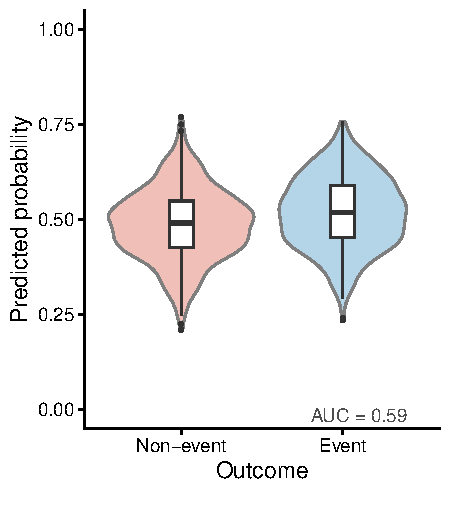
\includegraphics[width=\textwidth]{figures/Introduction/disc_poor.pdf}
    \caption{Poor}
    \label{fig:disc:poor}
\end{subfigure}
\hfill
\begin{subfigure}[b]{0.32\textwidth}
    \centering
    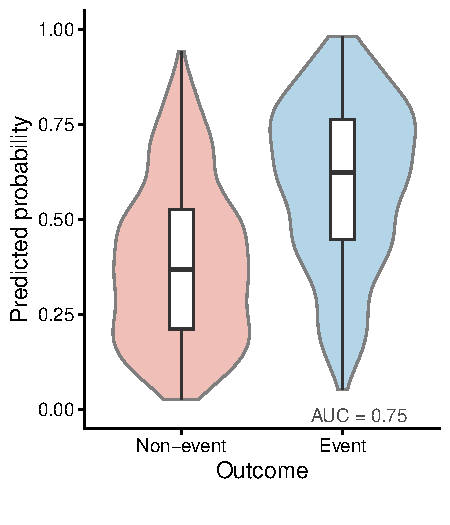
\includegraphics[width=\textwidth]{figures/Introduction/disc_moderate.pdf}
    \caption{Moderate}
    \label{fig:disc:moderate}
\end{subfigure}
\hfill
\begin{subfigure}[b]{0.32\textwidth}
    \centering
    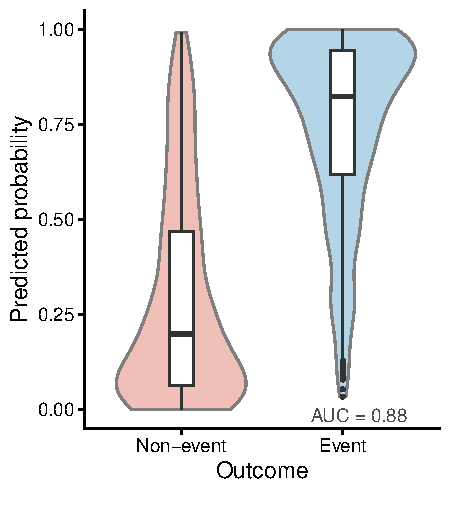
\includegraphics[width=\textwidth]{figures/Introduction/disc_good.pdf}
    \caption{Good}
    \label{fig:disc:good}
\end{subfigure}
\caption[Discrimination levels illustrated by violin plots]{Violin plots of predicted probabilities stratified by outcome group, illustrating three levels of discrimination. Red and blue represent non-events and events, respectively. The AUC increases from poor (a) to good (c) discrimination, reflecting greater separation between the two distributions. Note that poor, moderate, and good discrimination are relative terms that depend on the clinical context and the intended use of the model, rules of thumb about AUC values should be avoided.}
\label{fig:disc:levels}
\end{figure}

\subsection{Calibration}

\Gls{calibration} is the agreement between predicted probabilities and observed proportions.
In binary outcomes, the observed proportion of events needs to be estimated because the outcome is either 0 (non-event) or 1 (event). This can be done using different methods, such as \gls{binned calibration}, \gls{logistic_calibration}, or \gls{LOESS} smoothing (Figure~\ref{fig:cal:methods}). The logistic calibration framework characterises miscalibration through the intercept $\alpha$ and slope $\beta$ of the model $\text{logit}(p_{\text{obs}}) = \alpha + \beta \cdot \text{logit}(p_{\text{pred}})$, where $\alpha = 0$ and $\beta = 1$ indicate perfect calibration. Different combinations of $\alpha$ and $\beta$ correspond to distinct types of miscalibration (Figure~\ref{fig:miscal:types}).

Van Calster et al.\ \cite{vancalsterCalibrationHierarchyRisk2016} defined a hierarchy of four increasingly strict levels of calibration (Table~\ref{tab:intro:calhierarchy}). The most basic level is mean calibration, which requires that the average predicted probability equals the observed event rate. The next level is weak calibration, which requires that the calibration intercept $\alpha$ is 0 and the slope $\beta$ is 1 in the logistic calibration model \ref{fig:miscal:a0b1}. Then, moderate calibration requires that the observed event rate equals the predicted probability for every value of the predicted probability, which can be visualised using a flexible \gls{calibration_plot}. Flexible \glspl{calibration_plot} are created by smoothing the relationship between observed and predicted probabilities using a smoother of choice (e.g. \gls{LOESS} or \gls{restricted_cubic_splines}). Finally, strong calibration requires that the observed event rate equals the predicted probability for every covariate pattern, which is an idealised scenario that is practically impossible to achieve. 

\begin{table}[htbp]
\centering
\begin{threeparttable}
\caption[Calibration hierarchy for risk models]{Calibration hierarchy for risk models, based on Van Calster et al.\ \cite{vancalsterCalibrationHierarchyRisk2016}.}
\label{tab:intro:calhierarchy}
\small
\begin{tabularx}{\textwidth}{llXl}
\toprule
\textbf{Level} & \textbf{Name} & \textbf{Definition} & \textbf{Evaluation} \\
\midrule
1 & Mean & Average predicted probability equals the observed event rate & O:E ratio \\
2 & Weak & Calibration intercept $\alpha = 0$ and slope $\beta = 1$ & Logistic calibration framework \\
3 & Moderate  & $P(Y = 1 \mid \hat{p}) = \hat{p}$ for every $\hat{p}$ & Flexible calibration plot \\
4 & Strong & $P(Y = 1 \mid \mathbf{X}) = \hat{p}(\mathbf{X})$ for every covariate pattern $\mathbf{X}$ & Utopia \\
\bottomrule
\end{tabularx}
\end{threeparttable}
\end{table}



\begin{figure}[htbp]
\centering
\begin{subfigure}[b]{0.32\textwidth}
    \centering
    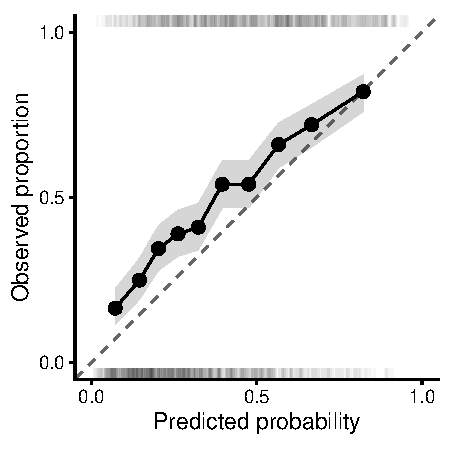
\includegraphics[width=\textwidth]{figures/Introduction/calibration_binned.pdf}
    \caption{Binned}
    \label{fig:cal:binned}
\end{subfigure}
\hfill
\begin{subfigure}[b]{0.32\textwidth}
    \centering
    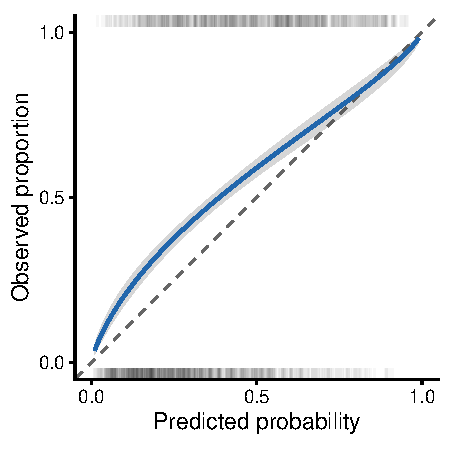
\includegraphics[width=\textwidth]{figures/Introduction/calibration_logistic.pdf}
    \caption{Logistic calibration}
    \label{fig:cal:logistic}
\end{subfigure}
\hfill
\begin{subfigure}[b]{0.32\textwidth}
    \centering
    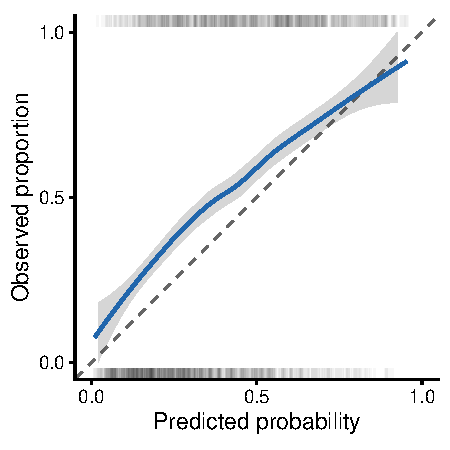
\includegraphics[width=\textwidth]{figures/Introduction/calibration_loess.pdf}
    \caption{LOESS}
    \label{fig:cal:loess}
\end{subfigure}
\caption[Calibration plots using binned, logistic, and LOESS methods]{Calibration plots for the same simulated data using three methods: (a) binned calibration, (b) logistic calibration, and (c) LOESS smoothed calibration curve. The dashed diagonal represents perfect calibration. Rug plots indicate the distribution of events (top) and non-events (bottom).}
\label{fig:cal:methods}
\end{figure}



\begin{figure}[htbp]
\captionsetup[subfigure]{font=scriptsize}
\centering
\begin{subfigure}[b]{0.32\textwidth}
    \centering
    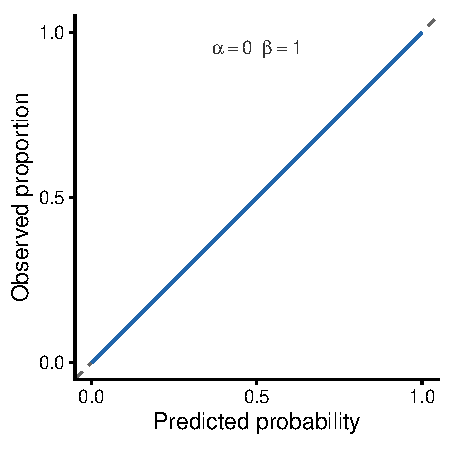
\includegraphics[width=\textwidth]{figures/Introduction/cal_a0_b1.pdf}
    \caption{Perfect calibration}
    \label{fig:miscal:a0b1}
\end{subfigure}
\hfill
\begin{subfigure}[b]{0.32\textwidth}
    \centering
    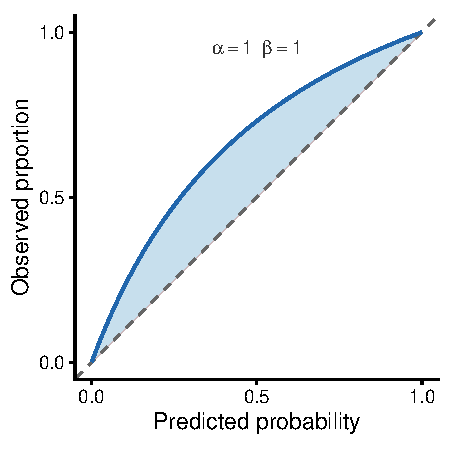
\includegraphics[width=\textwidth]{figures/Introduction/cal_a1_b1.pdf}
    \caption{Underestimation}
    \label{fig:miscal:a1b1}
\end{subfigure}
\hfill
\begin{subfigure}[b]{0.32\textwidth}
    \centering
    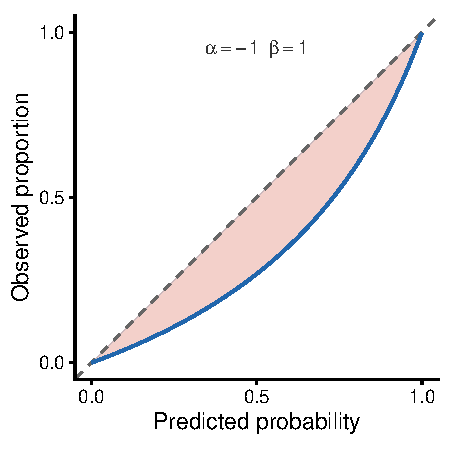
\includegraphics[width=\textwidth]{figures/Introduction/cal_am1_b1.pdf}
    \caption{Overestimation}
    \label{fig:miscal:am1b1}
\end{subfigure}

\vspace{0.5em}

\begin{subfigure}[b]{0.32\textwidth}
    \centering
    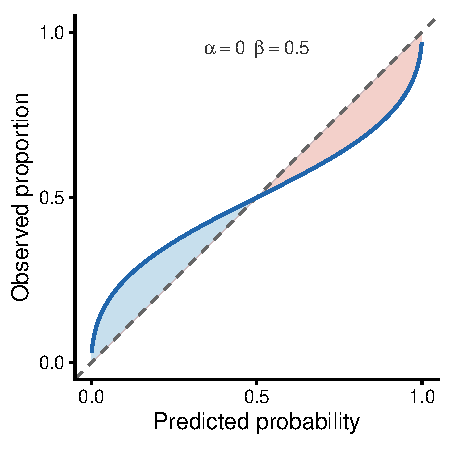
\includegraphics[width=\textwidth]{figures/Introduction/cal_a0_b05.pdf}
    \caption{\Gls{overfitting}}
    \label{fig:miscal:a0b05}
\end{subfigure}
\hfill
\begin{subfigure}[b]{0.32\textwidth}
    \centering
    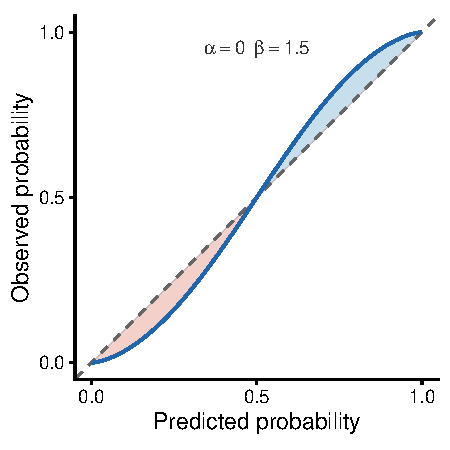
\includegraphics[width=\textwidth]{figures/Introduction/cal_a0_b15.pdf}
    \caption{\Gls{underfitting}}
    \label{fig:miscal:a0b15}
\end{subfigure}
\hfill
\begin{subfigure}[b]{0.32\textwidth}
    \centering
    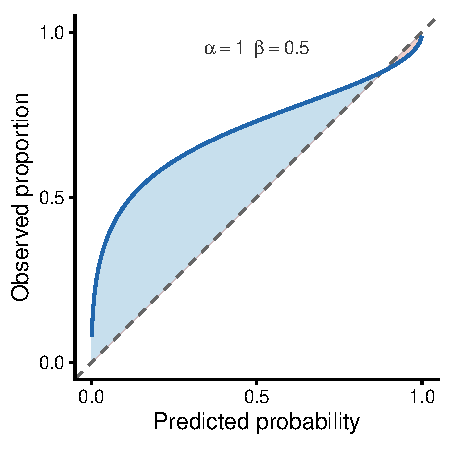
\includegraphics[width=\textwidth]{figures/Introduction/cal_a1_b05.pdf}
    \caption{Overfit + underestimation}
    \label{fig:miscal:a1b05}
\end{subfigure}

\vspace{0.5em}

\begin{subfigure}[b]{0.32\textwidth}
    \centering
    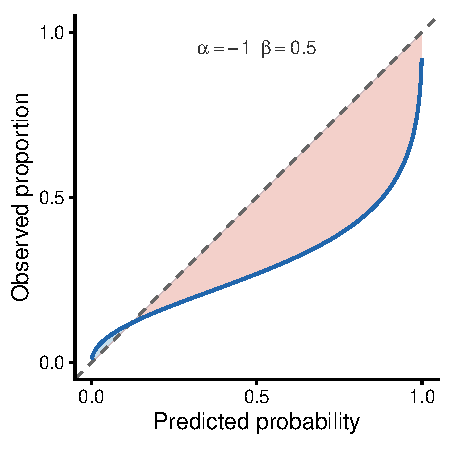
\includegraphics[width=\textwidth]{figures/Introduction/cal_am1_b05.pdf}
    \caption{Overfit + overestimation}
    \label{fig:miscal:am1b05}
\end{subfigure}
\hfill
\begin{subfigure}[b]{0.32\textwidth}
    \centering
    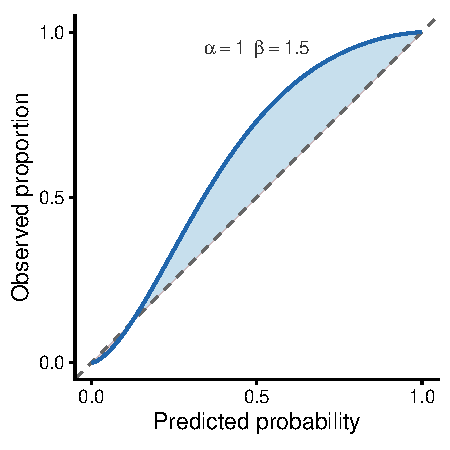
\includegraphics[width=\textwidth]{figures/Introduction/cal_a1_b15.pdf}
    \caption{Underfit + underestimation}
    \label{fig:miscal:a1b15}
\end{subfigure}
\hfill
\begin{subfigure}[b]{0.32\textwidth}
    \centering
    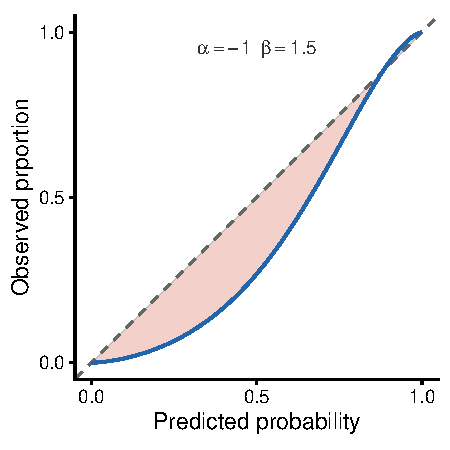
\includegraphics[width=\textwidth]{figures/Introduction/cal_am1_b15.pdf}
    \caption{Underfit + overestimation}
    \label{fig:miscal:am1b15}
\end{subfigure}

\caption[Types of miscalibration by calibration intercept and slope]{Types of miscalibration characterised by the calibration intercept $\alpha$ and slope $\beta$ in the logistic calibration framework $\text{logit}(p_{\text{obs}}) = \alpha + \beta \cdot \text{logit}(p_{\text{pred}})$. Blue shading indicates underestimation (observed $>$ predicted); red shading indicates overestimation (predicted $>$ observed). The dashed diagonal represents perfect calibration ($\alpha = 0$, $\beta = 1$).}
\label{fig:miscal:types}
\end{figure}

\subsection{Clinical utility}

\Gls{clinical_utility} refers to the quality of decisions that are informed by the model's predictions and is, arguably, the most important aspect of clinical model evaluation. It is a decision-analytic concept; therefore, it weighs the benefits of the model against misclassification costs. The main measure of \gls{clinical_utility} is \gls{net_benefit} (NB), which quantifies the balance between \glspl{true_positive} and \glspl{false_positive} at a given \gls{decision_threshold} \cite{vickersDecisionCurveAnalysis2006}. \Gls{NB} can be visualised using \gls{decision_curve_analysis}, which plots \gls{NB} across a range of decision thresholds to show the clinical value of using the model compared to default strategies of treating all patients or treating no patients, or compared with alternative models (Figure~\ref{fig:dca}). 

The \gls{decision_threshold} is independent of the prediction model and should reflect the clinical context and preferences, establishing the relation between the harms of treating healthy patients and the benefits of treating diseased patients \cite{onbehalfofthetopicgroupevaluatingdiagnostictestsandpredictionmodelsofthestratosinitiativeThreeMythsRisk2019}. This relation can differ across settings; therefore, the \gls{decision_threshold} should, too. For instance, a country with limited access to healthcare might set a higher threshold than a country with abundant resources, because the harm of treating healthy patients is higher in the former. A model that is clinically useful across a wide range of thresholds is more likely to be adopted in practice, as it can accommodate different clinical contexts and preferences \cite{vancalsterPerformanceEvaluationPredictive2024}.

\Gls{clinical_utility} is a first indication of the real-world impact of a prediction model, as it directly relates to patient outcomes and decision-making \cite{kappenEvaluatingImpactPrediction2018}. A model with excellent \gls{discrimination} and \gls{calibration} may still have limited \gls{clinical_utility} if the predicted probabilities do not lead to better decision-making. Conversely, a model with moderate \gls{discrimination} but good \gls{calibration} and high \gls{NB} at relevant thresholds can be highly valuable in practice. Therefore, evaluating \gls{clinical_utility} is essential to ensure that prediction models not only perform well statistically but also translate into meaningful improvements in patient care. 

\begin{figure}[htbp]
\centering
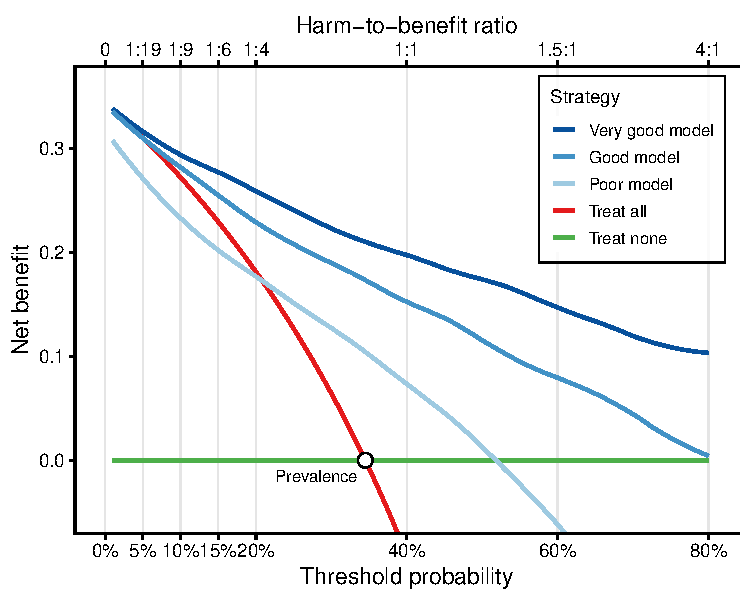
\includegraphics[width=0.8\textwidth]{figures/Introduction/dca.pdf}
\caption[Decision curve analysis for three simulated models]{Decision curve analysis for three simulated models with varying performance. At 10\% threshold, Model 1 (dark blue) and Model 2 (medium blue) provide \gls{NB} above both default strategies indicating clinical utility. Model 3 (light blue) is worse than treating all patients, therefore it would be harmful to use it in practice. \textbf{According to this decision curve analysis, Model 1 should be adopted in practice.} The top axis shows the corresponding harm-to-benefit ratio for each threshold probability.}
\label{fig:dca}
\end{figure}

\section{Developing a prediction model}

Developing a clinical prediction model involves a sequence of critical methodological steps, that are well explained in the literature \cite{steyerberg2019clinical, efthimiou_developing_2024,wynantsKeyStepsCommon2017}. Key questions that any prediction modeler should ask before developing a model are:
 
\begin{itemize}
    \item What is the clinical problem that the model is trying to solve?
    \item What is the target population for which the model is intended?
    \item What is the outcome that the model is trying to predict?
    \item What is the intended use of the model (e.g. diagnosis, prognosis, treatment selection)?
    \item Who will be the end-users of the model (e.g. clinicians, patients, healthcare systems)?
    \item What is the clinical context in which the model will be applied (e.g. primary care, hospital, low-resource settings)?
    \item What kind of predictors are available and routinely measured in the target population and setting?
\end{itemize}
    
These questions should have clear answers before any model is developed, because they will guide the whole process. However, before embarking on model development, the literature should be searched for existing models that might answer the same questions. This step is crucial to avoid unnecessary duplication of efforts and to build on existing knowledge \cite{smitsImprovingHealthCare2026}. 

\subsection{Develop a model or update an existing one?}

This is a fundamental question that any model developer needs to ask upfront. If there is a good quality model that has been developed for the same target population and with the same aim, it might be appropriate to first validate that model in your data. If the quality of the model is good, updating can be considered, which could entail recalibration, revision, or extension with new predictors \cite{vancalsterValidationUpdatingRisk2017}. If the quality of the existing model is low (e.g. high risk of bias), then developing a new model might be the best option. Developing a new model is more resource intensive and requires more expertise than updating an existing one; therefore, it should be considered only when there is a clear need. Publishing a new model without a clear justification contributes to the already large number of models in the literature and adds to the confusion among clinicians about which model to use \cite{arshiNumberPublicationsNew2025}. Once the need for a model is identified, we can proceed to the next steps of model development, which include variable selection, handling missing data, model specification and fitting, and validation.

\subsection{Variable selection and sample size}

The goal of variable selection is to identify the subset of predictors that will be included in the final model. Including too many predictors leads to unpractical models where too many characteristics need to be measured before obtaining a prediction. Variable selection is normally a priori guided by clinical knowledge and previous research. Then, data-driven variable selection occurs where statistical criteria are used to select the variables \cite{heinzeVariableSelectionReview2018}. Common statistical methods for variable selection in logistic regression include backward elimination or regularization techniques (e.g. Lasso, ridge), although they primarily rely on statistical properties such as p-values and information criteria (e.g. Akaike information criterion or Bayesian information criterion) which are unstable and can provide wrong results \cite{heinzeFiveMythsVariable2017}. This focus on statistical properties may not align with the ultimate goal of improving patient outcomes because the patient burden of measuring certain predictors is ignored. 

Variable selection should be guided by the intended use of the model and the clinical context in which it will be applied. For instance, if the model is intended to be used in a low-resource setting, then predictors that are not routinely measured in that setting should be avoided, even if they have good statistical properties in the development data. Collaboration with clinicians and other stakeholders is crucial to ensure that the selected predictors are relevant and feasible to measure in practice \cite{smitsImprovingHealthCare2026}. Variable selection algorithms that introduce the utilty of predictors in the selection process would be a solution to align variable selection with the ultimate goal of improving patient outcomes. 

\Gls{variable_selection} is closely related to sample size. Determining the sample size depends on several factors but the number of parameters in the model is a key one. The number of parameters depends on the candidate predictors; binary predictors require one parameter each, while categorical predictors with more than two categories require multiple parameters. For continuous predictors, if non-linearities are ignored, only one parameter is needed per predictor, but if non-linearities are modelled using splines or fractional polynomials, the number of parameters can increase substantially. In general, the more parameters in the model, the larger the sample size needed to avoid \gls{overfitting} and ensure reliable estimates. Flexible methods such as random forest or gradient boosting algorithms have shown to require larger sample sizes to avoid optimism \cite{vanderploegModernModellingTechniques2014,austinRelativeDataHungriness2024}.  

\subsection{Handling missing data}

Missing data is a common issue in clinical datasets and can lead to different types of bias if not handled properly. The most common approach is \gls{CCA}, which only includes patients with complete data for all predictors and the outcome \cite{eekhoutMissingDataSystematic2012}. This approach is pragmatic, but it can lead to biased estimates unless data is \gls{mcar_mechanism} (\gls{MCAR}), which is often unrealistic in clinical datasets \cite{vanderheijdenImputationMissingValues2006}. If possible, \gls{CCA} should be avoided because it reduces the available sample size \cite{Hughes2019}. A more robust approach is imputation, which fills in missing values based on observed data and typically assumes that missing data is \gls{mar_mechanism} (\gls{MAR}). Imputation can also be biased if the missingness follows \gls{mnar_mechanism} (\gls{MNAR}) pattern, where missingness depends on the unobserved value itself. A recommended approach for prediction models is multiple imputation, where missing values are imputed multiple times to create multiple complete datasets and properly account for imputation uncertainty \cite{siskImputationMissingIndicators2023}. Imputation decisions will affect the final model and the individual predictions and therefore should be based on careful consideration of the missingness reason, pattern and auxiliary information about missingness \cite{hughesAccountingMissingData2019}. If data are missing because a predictor is not routinely measured in the target population, excluding that predictor may be preferable to improve model applicability in practice.



\subsection{Model specification, fitting and internal validation}

Model specification involves choosing the functional form of the relationship between predictors and the outcome. For logistic regression, this typically involves deciding whether to include predictors as linear terms, to model non-linear relationships using splines or fractional polynomials, and whether to include interaction terms. For more complex models, such as deep learning, random forests or gradient boosting machines, model specification involves selecting the architecture and algorithm (e.g. number of layers and nodes in a neural network) and hyperparameters (e.g. learning rate, regularization strength). The process to select hyperparameters is called \gls{hyperparameter_tuning} and it is normally done by selecting the combination of hyperparameters that yields the best performance using \gls{bootstrap} or repeated \gls{cross_validation} among a grid of possible values for each hyperparameter  \cite{duniasComparisonHyperparameterTuning2024}. 

Then model fitting involves estimating the parameters of the model using the available data. For logistic regression, this is done using maximum likelihood estimation, which finds the parameter values that maximize the likelihood of observing the data given the model. For more complex models, such as deep learning, random forests or gradient boosting machines, fitting involves optimizing a loss function that measures the discrepancy between observed outcomes and predicted probabilities. In the bayesian framework, fitting involves specifying prior distributions for the parameters and updating these distributions based on the observed data \cite{vandeschootBayesianStatisticsModelling2021}. The choice of fitting method and model specification will affect both the performance and interpretability of the model.

Once the model is fitted, \gls{internal_validation} is the process of assessing the model's performance using the same data that was used for model development. This can be done using resampling techniques such as cross-validation or bootstrapping, which provide estimates of the model's performance that are less optimistic than the \gls{apparent_performance} obtained from the training data \cite{efthimiou_developing_2024,collinsEvaluationClinicalPrediction2024, dehondPerspectivesValidationClinical2023}. \Gls{internal_validation} is crucial to detect \gls{overfitting} and to obtain a more realistic estimate of how the model will perform on new data. However, it does not replace \gls{external_validation}, which is necessary to confirm that the model's performance generalizes to other populations and settings.

\section[Clustering in model development and evaluation]{Dealing with clustering in model development and evaluation}

\Glspl{clinical_prediction_model} are increasingly developed and validated using data from multiple centres or studies, generally known as clusters. An analysis of models in the Tufts  Predictive Analytics and Comparative Effectiveness (PACE) \gls{CPM} database found that 64\% of models developed after 2000 used multicenter data \cite{wynantsUntappedPotentialMulticenter2019}. Clustering introduces dependencies among patients within the same cluster, which can affect both model development and evaluation. Performance, particularly \gls{calibration}, varies across clusters due to differences in \gls{case_mix}, measurement practices, and local prevalence \cite{vancalsterValidationModelsDiagnose2020}. Ignoring clustering during validation can lead to misleading conclusions, as overall performance summaries may mask important \gls{heterogeneity} between clusters \cite{wynantsDoesIgnoringClustering2018}. Figure~\ref{fig:cal:clustering} illustrates this with a simulated example: the overall calibration curve obtained by combining the data from two clusters lies on the diagonal, suggesting excellent \gls{calibration}, while the cluster-specific curves reveal substantial miscalibration in opposite directions. For these reasons, methods that account for clustering when developing and evaluating \glspl{clinical_prediction_model} should be developed and adopted, particularly for calibration \cite{debrayFrameworkMetaanalysisPrediction2019,debrayTransparentReportingMultivariable2023}. These include meta-analytic techniques to summarise performance across clusters (e.g. \gls{IPD} meta-analysis), and a comprehensive analysis of the between-cluster \gls{heterogeneity} as outlined in the \gls{TRIPOD}-Cluster guideline.

\begin{figure}[htbp]
\centering
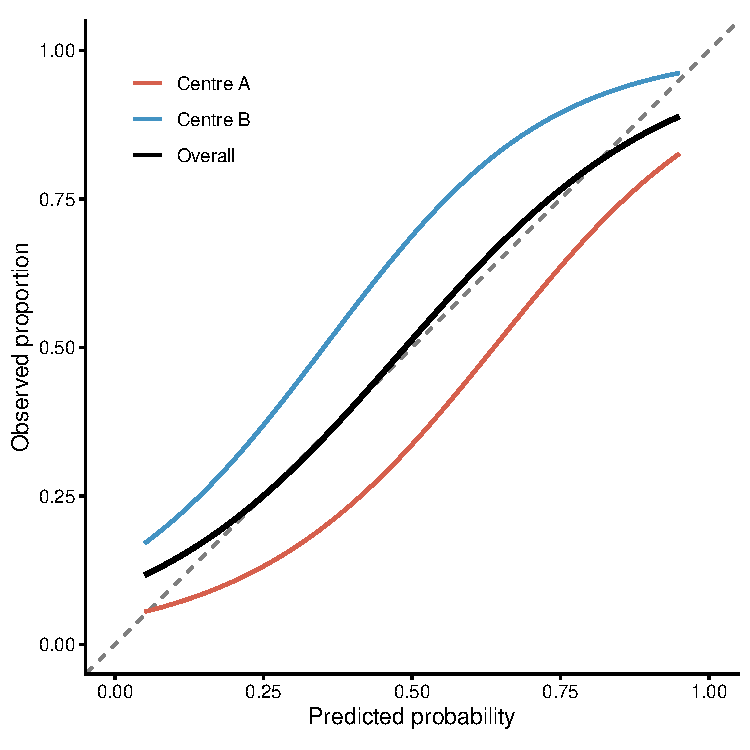
\includegraphics[width=0.6\textwidth]{figures/Introduction/calibration_clustering.pdf}
\caption[Clustering masking miscalibration in calibration curves]{Simulated calibration curves illustrating how clustering can mask miscalibration. The overall curve (black) appears perfectly calibrated, but centre-specific curves reveal that Centre A (red) overestimates and Centre B (blue) underestimates the observed event rate.}
\label{fig:cal:clustering}
\end{figure}


\subsection{Meta-analysis and heterogeneity}

The previous section highlighted that ignoring clustering can mask important differences in model performance across centres. When a prediction model is validated in multiple clusters, whether centres in a multicentre study or studies in a systematic review, each cluster might have a different performance in terms of \gls{AUC}, \gls{calibration_intercept}, \gls{observed_expected_ratio} or \gls{NB}. These cluster-specific performances can be formally synthesised using \gls{random_effects_meta_analysis} \cite{debrayGuideSystematicReview2017,debrayFrameworkMetaanalysisPrediction2019}. In this framework, each cluster's true performance is assumed to be drawn from a distribution with overall mean $\mu$ and between-cluster variance $\tau^2$. We assume that there is \gls{heterogeneity} and that there is no single 'true' performance; instead, the true performance varies across clusters. The pooled estimate represents the expected performance in a typical cluster, while $\tau^2$ captures how much the true performance varies across clusters beyond what is expected from sampling variability alone.

% In the context of \gls{IPD} meta-analysis, where patient-level data are available from each cluster, the within-cluster and between-cluster variance components can be estimated more precisely than in aggregate data meta-analysis \cite{rileyIndividualParticipantData2021a}. 
The pooled estimate is obtained as a weighted average of the cluster-specific estimates, where weights reflect both the within-cluster variance ($\sigma_j^2$) and the estimated between-cluster variance ($\tau^2$). Several frequentist estimation methods exist for $\tau^2$, including \gls{DL}, \gls{REML}, and \gls{PM} \cite{veronikiMethodsEstimateBetweenstudy2016}. \Glspl{CI} for the pooled estimates can be obtained using the normal approximation, or using the \gls{HKSJ} adjustment, which accounts for the uncertainty in estimating $\tau^2$ and provides better control of type I error rates when the number of clusters is small \cite{inthoutHartungKnappSidikJonkmanMethodRandom2014}.

Beyond the pooled estimate, understanding and quantifying \gls{heterogeneity} is central to interpreting the results of a meta-analysis. Several complementary measures are available, each capturing a different aspect of \gls{heterogeneity} (Table~\ref{tab:intro:heterogeneity}). The between-cluster variance $\tau^2$ is the fundamental \gls{heterogeneity} parameter and its square is on the scale of the performance metric being pooled. The $I^2$ statistic expresses the proportion of total variability attributable to between-cluster \gls{heterogeneity} rather than sampling error \cite{higginsQuantifyingHeterogeneityMetaanalysis2002}. Although $I^2$ is widely reported, it depends on within-cluster precision and can be misleadingly high when studies included in the meta-analysis are large or misleadingly low when studies included in the meta-analysis are small, even when the absolute \gls{heterogeneity} ($\tau^2$) is the same \cite{steyerbergAssessmentHeterogeneityIndividual2019}. Cochran's $Q$ tests the null hypothesis of no \gls{heterogeneity}, but has low statistical power when few clusters are available. For these reasons, the \gls{prediction_interval} is arguably the most clinically informative summary: it estimates the range within which the performance of the model is expected to fall in a new, similar cluster \cite{higginsReevaluationRandomeffectsMetaanalysis2009,partlettRandomEffectsMetaanalysis2017}. The most common approach to obtaining the \gls{prediction_interval} was introduced by Higgins et al. \cite{higginsReevaluationRandomeffectsMetaanalysis2009}. It combines the pooled estimate, its standard error, and the estimated $\tau^2$ to form the interval $\hat{\mu} \pm t_{k-2, 1-\alpha/2} \sqrt{\text{SE}(\hat{\mu})^2 + \tau^2}$, where $t_{k-2, 1-\alpha/2}$ is the $1-\alpha/2$ percentile of the $t$-distribution with $k-2$ degrees of freedom and $k$ is the number of clusters. With $\alpha = 0.05$, the resulting 95\% \gls{prediction_interval} indicates the range within which the true performance of a hypothetical new cluster is expected to fall. However, this frequentist approximation has been shown to perform well only when \gls{heterogeneity} is substantial and cluster sample sizes are reasonably similar \cite{partlettRandomEffectsMetaanalysis2017}. 

As an alternative to frequentist methods, Bayesian \gls{random_effects_meta_analysis} places a prior distribution on all meta-analysis parameters, including $\tau^2$, and estimates the posterior distribution of the pooled effect; this approach naturally incorporates the full uncertainty about $\tau^2$ into both the \gls{CrI} for the pooled estimate and the \gls{prediction_interval} for a new cluster, but requires specification of prior distributions and more computational resources \cite{higginsReevaluationRandomeffectsMetaanalysis2009}. In Bayesian meta-analysis, the \gls{prediction_interval} can be directly derived from the posterior predictive distribution of the pooled effect and $\tau^2$ and it is recommended because it ensures that the model accounts for the uncertainty of estimating $\text{SE}(\hat{\mu})^2$ and $\tau^2$ \cite{debrayFrameworkMetaanalysisPrediction2019} .

\begin{table}[htbp]
\centering
\caption[Heterogeneity measures in random effects meta-analysis]{Summary of heterogeneity measures in random effects meta-analysis of prediction model performance.}
\label{tab:intro:heterogeneity}
\begin{tabularx}{\textwidth}{>{\raggedright\arraybackslash}p{0.22\textwidth} >{\raggedright\arraybackslash}X >{\raggedright\arraybackslash}X}
\toprule
\textbf{Measure} & \textbf{Definition} & \textbf{Interpretation} \\
\midrule
% Within-cluster variance ($\sigma_j^2$) & Sampling variability of the performance estimate within cluster $j$ & Reflects the precision of the cluster-specific estimate; decreases with larger sample sizes \\
% \addlinespace
Between-cluster variance ($\tau^2$) & Variance of the true underlying performance across clusters & Core heterogeneity parameter; represents variability in true performance beyond sampling error \\
\addlinespace
$I^2$ & Proportion of total variability due to between-cluster heterogeneity: $\tau^2 / (\tau^2 + \tilde{\sigma}^2)$ & Ranges from 0\% to 100\%; depends on study precision and should not be interpreted in isolation \\
\addlinespace
Cochran's $Q$ & Weighted sum of squared deviations of cluster estimates from the pooled estimate & Tests the null hypothesis of no heterogeneity; low power with few clusters \\
\addlinespace
95\% Prediction interval & Interval for the expected performance in a new cluster & Incorporates both uncertainty in the pooled mean and $\tau^2$; directly relevant for generalisability \\
\bottomrule
\end{tabularx}
\end{table}

Figure~\ref{fig:forest:methods} illustrates a simulated random effects meta-analysis of the \gls{AUC} across ten studies, comparing these estimation approaches. While the pooled point estimates are nearly identical across methods, the HKSJ adjustment consistently widens the confidence interval relative to the standard interval for a given $\tau^2$ estimator. The Bayesian approach yields the widest prediction interval, reflecting its fuller accounting of uncertainty in $\tau^2$. Across all methods, the 95\% prediction intervals are substantially wider than any confidence interval, illustrating that the expected performance in a new setting is far more uncertain than the estimated mean performance.

\begin{figure}[htbp]
\centering
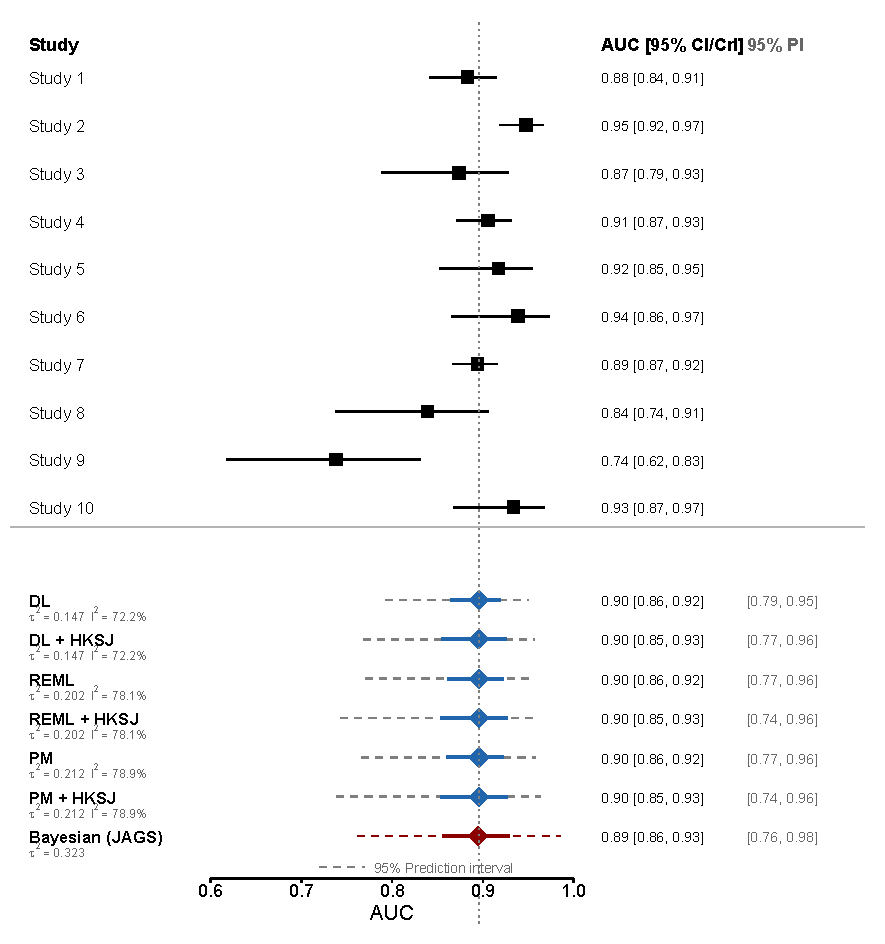
\includegraphics[width=0.85\textwidth]{figures/Introduction/forest_meta_methods.pdf}
\caption[Forest plot comparing meta-analysis estimation methods]{Forest plot of the AUC from ten simulated studies pooled using seven random effects meta-analysis approaches: three $\tau^2$ estimators (DerSimonian-Laird, REML, Paule-Mandel) each with standard and HKSJ-adjusted confidence intervals, and a Bayesian approach with a 95\% \gls{CrI}. Black squares: study-specific estimates with 95\% confidence intervals. Blue diamonds: frequentist pooled estimates. Red diamond: Bayesian pooled estimate using \texttt{metamisc} \cite{metamisc}. Solid lines: 95\% confidence or \glspl{CrI}. Dashed lines: 95\% prediction intervals.}
\label{fig:forest:methods}
\end{figure}

% In this thesis, random effects meta-analysis with $\tau^2$ and 95\% \glspl{PI} is used in the systematic reviews of \gls{ADNEX} performance (Chapters~\ref{sec:chp_ADNEXSR} and~\ref{sec:chp_ADNEXvsRMI}). Chapter~\ref{sec:chp_ClusteredCalibration} extends the quantification of heterogeneity to calibration curves, where prediction intervals indicate, for every predicted risk, the range of observed proportions expected in a new cluster. This shift from scalar summaries to heterogeneity across the full calibration curve provides a richer picture of how well a model generalises.
% }
\subsection{Mixed models}

Another approach to deal with clustering when developing or validating a prediction model are \glspl{mixed_effects_model} (also known as multilevel or hierarchical models) \cite{snijdersMultilevelAnalysisIntroduction2012,wynantsUntappedPotentialMulticenter2019}. These models include fixed effects, which capture the overall relationship between predictors and outcome, and random effects, which capture cluster-specific deviations from this overall relationship. For a binary outcome, a mixed effects logistic regression with a \gls{random_intercept} per cluster $j$ takes the form
\begin{equation}
\text{logit}(p_{ij}) = \beta_0 + \boldsymbol{\beta}^T \mathbf{x}_{ij} + u_j, \quad u_j \sim \mathcal{N}(0, \tau^2),
\end{equation}
where $p_{ij}$ is the probability of the event for patient $i$ in cluster $j$, $\boldsymbol{\beta}^T \mathbf{x}_{ij}$ represents the fixed predictor effects, and $u_j$ is the cluster-specific \gls{random_intercept} drawn from a normal distribution with variance $\tau^2$. The \gls{random_intercept} allows the baseline risk to vary across clusters. The model can be extended with \glspl{random_slope} to allow the effect of one or more predictors to vary across clusters as well. If only a \gls{random_intercept} is included, only one extra parameter (the between-cluster variance $\tau^2$) is added to the model, regardless of the number of clusters. In contrast, a fixed effects model (i.e. logistic regression) with a separate intercept for each cluster would require $k-1$ additional parameters. If random slopes are included, the number of parameters increases with the number of predictors that have random effects, but it still remains more parsimonious than a fixed effects model with separate cluster-predictor interactions.

When including random effects cluster-specific estimates are shrunk towards the overall estimate due to the \gls{shrinkage} factor. This \gls{shrinkage} is determined by the between-cluster variability, within cluster variability and the number of observations per cluster. Bigger clusters that are similar to the overall estimate exhibit less \gls{shrinkage}, while smaller clusters or clusters with more extreme estimates are more heavily shrunk \cite{wynantsDoesIgnoringClustering2018}. This is desirable: it borrows information across clusters rather than treating each one in isolation, which would be imprecise for small clusters, or ignoring clustering entirely, which would mask between-cluster \gls{heterogeneity}. These estimates are called \gls{empirical_bayes_estimates} because they can be interpreted as the posterior mean of the cluster-specific effect given the observed data and the estimated variance components \cite{snijdersMultilevelAnalysisIntroduction2012}.

In Figure~\ref{fig:intro:mixedmodels} the effect of ignoring clustering is illustrated. The left panel shows the cluster-specific calibration curves from a standard logistic regression that ignores clustering, while the right panel shows the curves from a mixed effects logistic regression with \glspl{random_intercept}. The simulated data consist of six clusters that differ in baseline risk, which is captured by the random intercepts in the mixed model. Ignoring clustering leads to predictions that do not reflect these different baseline risks, resulting in poor cluster-specific calibration. In contrast, the mixed effects model adjusts for these differences, bringing the cluster-specific calibration curves much closer to the diagonal, indicating better calibration within each cluster. Flexible calibration curves are recommended according to Van Calster et al. (Table~\ref{tab:intro:calhierarchy}), but currently there is no method to fit flexible calibration curves that account for clustering.


\begin{figure}[htbp]
\centering
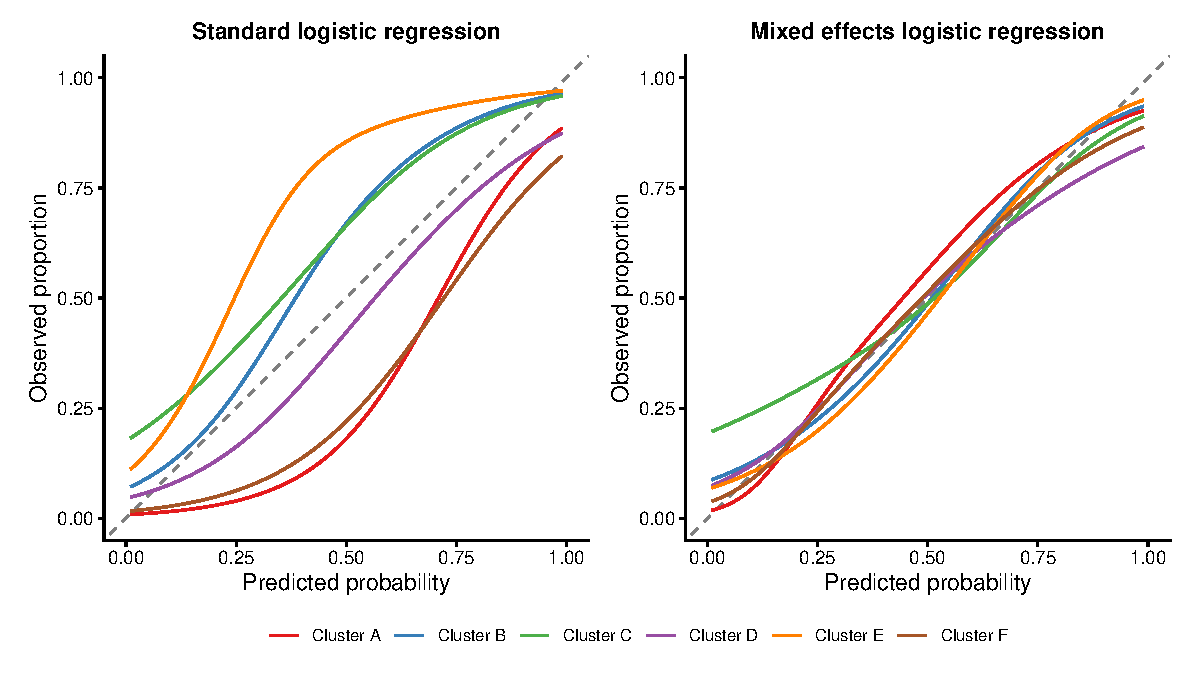
\includegraphics[width=\textwidth]{figures/Introduction/mixed_models.pdf}
\caption[Calibration comparison: standard vs.\ mixed effects logistic regression]{Cluster-specific calibration curves from simulated data with six clusters that differ in baseline risk. (Left)~A standard logistic regression ignoring clustering produces predictions that are poorly calibrated within individual clusters. (Right)~A mixed effects logistic regression with random intercepts adjusts for cluster-specific baseline risks, resulting in calibration curves that are closer to the diagonal.}
\label{fig:intro:mixedmodels}
\end{figure}

Mixed models do require more complex estimation procedures and distributional assumptions (typically normality of the random effects), which should be carefully considered \cite{snijdersMultilevelAnalysisIntroduction2012}. 


\section{Can we predict individual risks?}
\begin{quote}
    \textit{In our everyday world, probability probably does not exist -- but it is often useful to act as if it does --- David Spigelhalter, 2024 \cite{spiegelhalterWhyProbabilityProbably2024}}
\end{quote}


The ultimate goal of a \gls{clinical_prediction_model} is to provide an accurate estimate of the risk of a specific outcome for an individual patient that can help with medical decision-making. This risk estimate is calculated by applying the model to the patient's data, which involves plugging in the patient's predictor values into the model's equation to obtain a predicted probability. For example, in a logistic regression model, the predicted probability of the event for a patient is calculated as $p = \text{logit}^{-1}(\beta_0 + \boldsymbol{\beta}^T \mathbf{X})$, where $\beta_0$ is the intercept, $\boldsymbol{\beta}$ is the vector of predictor coefficients, and $\mathbf{X}$ is the vector of the patient's predictor values. For more complex models, such as random forests or neural networks, the predicted probability is obtained by applying the model's algorithm to the patient's data. However, in real life, we will never know the true individual risk for a patient: the patient will either experience the event (or condition) or not. This classic problem was first introduced by John Venn in 1876, where he stated that everything (every event) has infinite measurable characteristics and can therefore be considered as belonging to an indefinite number of classes or groups \cite{Venn1876}. This was the foundation of the "reference class problem", which states that the risk of an individual patient can vary depending on the group to which they are assigned \cite{Reichenbach1949}. For instance, a patient might have a 10\% risk of developing a certain disease based on their age and sex, but if we also consider their family history, the risk might increase to 20\%, and both risks can be correct. This problem highlights the importance of providing and understanding the uncertainty around the individual risks. This uncertainty is commonly presented in the form of a \gls{CI} for the predicted probability, which quantifies the range of values within which the true risk is expected to lie with a certain level of confidence (e.g. 95\%). A more recent approach to quantify this uncertainty is through the effective sample size, which estimates the number of patients in the development data that are effectively similar to the patient for whom the risk is being predicted \cite{thomassenEffectiveSampleSize2025}. However, these approaches do not take into account the reference class problem, and assume that the selected model is the correct one and that the patient belongs to a single reference class whereas the total uncertainty remains unknown and potentially underestimated. Although individual risks might be inherently unknowable and no model can be accurately predict risk for all individuals, if a model presents good population level performance in terms of discrimination, calibration and clinical utility, this implies that the model will be a valuable tool for public health. 

\section[Enhancing quality of prediction model research]{The EQUATOR network and the STRATOS initiative: enhancing the quality of prediction model research}
 
The \gls{EQUATOR} network is an international network that seeks to improve the quality of health research by promoting transparent and accurate reporting and adherence to robust reporting guidelines \cite{simeraTransparentAccurateReporting2010}. The \gls{STRATOS} initiative is a related effort that provides guidance on the design, analysis, and reporting of observational studies, including those developing and validating prediction models \cite{sauerbreiSTRengtheningAnalyticalThinking2014}. \gls{STRATOS} aims to produce both accessible guidance for researchers with low statistical knowledge and detailed guidance for experts in different areas related to observational studies.

Transparent and complete reporting of prediction model studies is essential for assessing the quality and applicability of published models. The \gls{TRIPOD} and its update \gls{TRIPOD}+AI statements provide a checklist of items that should be reported in studies developing, validating, or updating a prediction model \cite{collinsTransparentReportingMultivariable2015,collinsTRIPODAIStatementUpdated2024}. A recent extension, \gls{TRIPOD}-SRMA, addresses reporting for systematic reviews and meta-analyses of prediction model studies \cite{snellTransparentReportingMultivariable2023}. To handle the growing use of multicenter data, \gls{TRIPOD}-Cluster was published to guide the reporting of studies that develop or validate models using clustered data \cite{debrayTransparentReportingMultivariable2023}. For the analysis of risk of bias \gls{PROBAST} and its update PROBAST+AI provide a structured tool to assess the risk of bias and applicability of prediction model studies \cite{moonsPROBASTToolAssess2019, moonsPROBASTAIUpdatedQuality2025}.

\gls{STRATOS} has provided detailed guidance about performance measures, \cite{vancalsterPerformanceEvaluationPredictive2024} variable selection \cite{heinzeVariableSelectionReview2018},  simulation studies \cite{boulesteixIntroductionStatisticalSimulations2020}, handling missing data \cite{leeFrameworkTreatmentReporting2021} and methodological research \cite{heinzePhasesMethodologicalResearch2024} among other topics. The whole published guidance can be found in the STRATOS website (\url{https://www.stratos-initiative.org}) and it is an invaluable resource for researchers developing and validating prediction models. 

These guidelines and recommendations play a crucial role in improving the quality and reproducibility of prediction modelling research.


\section{Medical device regulation}

\Glspl{CPM} deployed as software tools are subject to medical device regulation. Under the European Union \gls{MDR} (EU 2017/745), software intended for medical purposes --- including diagnosis, prediction, and prognosis --- is explicitly classified as a medical device, even when it operates independently of any hardware \cite{EUMDR2017}. Similarly, the U.S. Food and Drug Administration regulates such tools under the \gls{SaMD} framework and has authorised over 1,000 AI/ML-enabled devices to date \cite{FDA_AIML_SaMD_2021}. The more recent EU Artificial Intelligence Act (EU 2024/1689) introduces additional requirements for high-risk AI systems, which include most medical AI applications \cite{EUAIAct2024}. These regulatory frameworks reinforce the need for rigorous model development, thorough external validation, and continuous post-market monitoring. These principles align closely with the methodological standards discussed throughout this thesis and support the development of trustworthy AI in healthcare. However, the monetary cost of compliance with these regulations can be prohibitive, especially for academic researchers, who might need to commercialise models to cover these costs \cite{kotlarzImpactMedicalDevice2025}. The misalignment between open science principles and current medical device regulation is a significant challenge that needs to be addressed to ensure that valuable prediction models can be safely, widely, and fairly adopted in clinical practice without compromising transparency and accessibility \cite{van2026enemies}.

\section{IOTA and ovarian masses}

Adnexal masses, which include ovarian tumours and other masses arising from the ovary or surrounding structures, are a common finding in gynaecological practice. In 2022 more than 300,000 new cases of ovarian cancer were diagnosed worldwide with more than 200,000 deaths. This makes ovarian cancer the eighth most deadly cancer in the world \cite{brayGlobalCancerStatistics2024}. In Europe the trend for ovarian cancer mortality is positive, and it is expected to keep reducing in the near future \cite{wojtylaEuropeanTrendsOvarian2023}. Most adnexal masses are benign, and only a minority turn out to be malignant. Because the optimal management of a patient with an adnexal mass depends on the histological type of the mass, accurate preoperative characterisation is essential.

Patients with a benign mass can be managed conservatively with clinical and ultrasound follow-up, or treated with minimally invasive surgery (i.e. robotic or human laparoscopy) \cite{carleyLaparoscopyLaparotomyManagement2002, froymanRiskComplicationsPatients2019}. In contrast, patients with a malignant mass benefit from management in specialised oncology centres, and the specific surgical approach may differ depending on the malignant subtype \cite{wooCentralisationServicesGynaecological2012, timmermanESGOISUOGIOTA2021}. Borderline tumours, early-stage primary invasive tumours, advanced primary invasive tumours, and secondary metastatic tumours each require different treatment pathways. To optimise patient triage without operating on all patients, diagnostic tools that can estimate the likelihood of malignancy from preoperative information are needed.

Transvaginal ultrasound is the primary imaging modality for characterising adnexal masses. The \gls{IOTA} group is a multinational research collaboration founded in 1999 dedicated to improving the preoperative characterisation of adnexal masses through standardised ultrasound assessment. The group began by establishing consensus definitions and measurement rules for ultrasound features \cite{timmermanTermsDefinitionsMeasurements2000}, which standardised the sonographic description of adnexal tumours and served as the foundation for systematic data collection across centres, and were updated 26 years later \cite{timmermanTermsDefinitionsMeasurements2026}.

Since then, the \gls{IOTA} group has conducted a series of large-scale prospective studies (\gls{IOTA} phases 1 through 7), collecting standardised clinical and ultrasound data from more than 30,000 patients with adnexal masses at centres across multiple countries. These datasets have served as the basis for developing and validating several evidence-based diagnostic models. The following section details the specific models and tests developed to determine the preoperative management of adnexal masses, within the IOTA group and outside of it.

\section{Models and tests to diagnose ovarian masses}

A multitude of mathematical models and scoring systems have been proposed over the years to support the preoperative characterisation of adnexal masses (Table~\ref{tab:intro:models}). However, a comprehensive systematic review by Kaijser et al.\ \cite{kaijserPresurgicalDiagnosisAdnexal2014} highlighted that the majority of these models suffered from poor methodological quality, small development datasets, and a lack of independent external validation. Among the tools that have demonstrated clinical utility, the \gls{RMI}, published in 1990, was one of the first to be widely adopted \cite{jacobsRiskMalignancyIndex1990}. The \gls{RMI} combines a serum CA-125 level, menopausal status, and five binary ultrasound features into a single score. A threshold (commonly 200) is used to classify tumours as high or low risk for malignancy. Despite being developed on data from only 143 patients at a single hospital, the \gls{RMI} has been widely adopted and remains recommended by several national clinical guidelines \cite{timmermanESGOISUOGIOTA2021}. Another widely used scoring system created by the American College of Radiology is \gls{ORADS}-US, which classifies tumours into five categories based on ultrasound features, with each category corresponding to a different risk of malignancy and recommended management strategy \cite{andreottiORADSUSRisk2020}. 

Biomarkers have also been proposed to support the diagnosis of ovarian cancer. The most widely used biomarker is CA-125, which is associated with ovarian cancer but is not good at distinguishing between benign and malignant tumours on its own \cite{mossRoleCA125Clinical2005}. The ROMA algorithm combines CA-125 with HE4 and menopausal status to estimate the risk of malignancy \cite{mooreUseMultipleNovel2008}. CA72.4 and CA15.3 have also been proposed to discriminate between malignant subtypes \cite{coosemansAddedValueSerum2025}, but cell-free DNA biomarkers have not yet been shown to be clinically useful for the preoperative characterisation of adnexal masses \cite{vandersticheleAddedValueCellfree2025}. 

The \gls{IOTA} group developed several diagnostic tools building on their standardised prospective studies. The \gls{IOTA} Simple Rules use ten ultrasound features (five suggestive of malignancy and five suggestive of a benign mass) to classify tumours without requiring a calculation \cite{timmermanSimpleUltrasoundbasedRules2008}. Years later, these rules were converted into a logistic regression model (the SRRisk model) \cite{timmermanPredictingRiskMalignancy2016}. The \gls{IOTA} logistic regression models (\gls{LR1} and \gls{LR2}) estimate the probability of malignancy using logistic regression with ultrasound and clinical variables \cite{timmermanLogisticRegressionModel2005}. In 2012, the IOTA group presented the Benign Simple Descriptors, a set of four ultrasound features that are highly specific for benign tumours and can be used to rule out malignancy without the need for a risk calculation \cite{ameyeClinicallyOrientedThreeStep2012}. 

\subsection{ADNEX model}

Built on the knowledge obtained through previous studies in 2014 the IOTA group published the most comprehensive model, the \gls{ADNEX} model \cite{vancalsterEvaluatingRiskOvarian2014}. Unlike earlier models that distinguish only between benign and malignant masses, \gls{ADNEX} is a multinomial logistic regression model that estimates the probability of five tumour types: benign, borderline, stage I primary invasive, stage II--IV primary invasive, and secondary metastatic. The model uses three clinical predictors (age, serum \gls{CA125}, and type of centre) and six ultrasound variables (maximal diameter of the lesion, proportion of solid tissue, number of papillary projections, presence of more than 10 cyst locules, acoustic shadows, and ascites). A version without \gls{CA125} is also available for settings where the serum marker is not routinely measured. \gls{ADNEX} was developed using data from 5909 patients who underwent surgery at 24 centres across 10 countries. 

Van Calster et al.\ \cite{vancalsterValidationModelsDiagnose2020} conducted the largest prospective external validation to date, comparing six diagnostic models in 4905 patients across 17 centres. \gls{ADNEX} (with and without \gls{CA125}) and \gls{SRRisk} achieved the highest discrimination (\gls{AUC} 0.94), while \gls{RMI} had the lowest (\gls{AUC} 0.89). Calibration varied across centres for all models. The latest recommendation is the two-step strategy, where the Benign Descriptors are applied first to identify clearly benign masses (applicable in 37\% of masses where 99.3\% were benign), and then \gls{ADNEX} is applied to the remaining masses \cite{landolfoBenignDescriptorsADNEX2023}. The main limitation of the ADNEX model is that it was developed on patients who underwent surgery, which may not be representative of the full spectrum of patients with adnexal masses, especially those managed conservatively. Updating or refitting the model using data from patients managed conservatively could improve its generalisability to this broader population.

\begin{table}[t]
\centering
\footnotesize
\setlength{\tabcolsep}{4pt}
\caption[Diagnostic models and tests for adnexal masses]{Non exhaustive overview of diagnostic models and tests for preoperative diagnosis of adnexal masses. In bold ADNEX model predictors; US = ultrasound.}
\label{tab:intro:models}
\begin{tabularx}{\textwidth}{@{} l c >{\raggedright\arraybackslash}X >{\raggedright\arraybackslash}X @{}}
\toprule
\textbf{Model/Test} & \textbf{Year} & \textbf{Predictors (n)} & \textbf{Notes} \\
\midrule
\multicolumn{4}{@{}l}{\textit{Prediction models (probabilistic output)}} \\
\addlinespace
LR1 \cite{timmermanLogisticRegressionModel2005} & 2005 & Personal history of ovarian cancer, hormonal therapy, \textbf{age}, \textbf{max.\ diameter of the lesion}, pain, \textbf{ascites}, \textbf{papillary flow}, entirely solid tumour, max.\ diameter of the solid part, irregular walls, \textbf{shadows}, colour score (9) & Logistic regression \\
\addlinespace
LR2 \cite{timmermanLogisticRegressionModel2005} & 2005 & \textbf{Age}, \textbf{ascites}, blood flow, max.\ diameter of the solid part, irregular walls, \textbf{shadows} (6) & Simplified version of LR1 \\
\addlinespace
ROMA \cite{mooreUseMultipleNovel2008} & 2008 & HE4, \textbf{CA-125}, menopausal status (3) & Serum biomarker algorithm \\
\addlinespace
ADNEX \cite{vancalsterEvaluatingRiskOvarian2014} & 2014 & \textbf{Age}, \textbf{CA-125}, \textbf{centre type}, \textbf{max.\ diameter lesion},\textbf{proportion of solid tissue}, \textbf{papillary projections}, \textbf{$>$10 locules}, \textbf{shadows}, \textbf{ascites} (9) & Multinomial logistic regression (Benign, Borderline, Stage I, Stage II-IV and Metastatic) \\
\addlinespace
SRRisk \cite{timmermanPredictingRiskMalignancy2016} & 2016 & Simple Rules features + \textbf{type of center} & Logistic regression. Adaptation of simple rules to a probabilistic approach \\
\addlinespace
Two-step strategy \cite{landolfoBenignDescriptorsADNEX2023} & 2023 & Step 1: BDs; Step 2: \textbf{ADNEX} & BDs applicable in 37\% of masses where 99.3\% were benign \\
\midrule
\multicolumn{4}{@{}l}{\textit{Tests and rules (classification)}} \\
\addlinespace
RMI \cite{jacobsRiskMalignancyIndex1990} & 1990 & \textbf{CA-125}, menopausal status, US score (5 binary features) & Score-based; threshold commonly 200 \\
\addlinespace
Simple Rules \cite{timmermanSimpleUltrasoundbasedRules2008} & 2008 & 10 binary US features (5 Benign rules + 5 Malignant rules) & If only benign rules apply, the tumour is deemed benign and vice versa. Applicable to $\sim$76\% of the masses.  \\
\addlinespace
Benign Descriptors \cite{ameyeClinicallyOrientedThreeStep2012} & 2012 & 4 benign US patterns (e.g.\ unilocular cyst, typical dermoid, typical endometrioma) & Triage tool to identify clearly benign masses from which 99.3\% were benign \\
\addlinespace
O-RADS \cite{andreottiORADSUSRisk2020} & 2020 & US morphological features (IOTA lexicon) or ADNEX risk & Risk categories (0--5)\\
\addlinespace
CA-125 & --- & Serum \textbf{CA-125} level & Threshold commonly 35~U/mL \\
\addlinespace
Subjective Assessment & --- & Expert US pattern recognition & Depends on examiner experience \\
Histopathology & --- & Microscopic examination of tissue samples & Gold standard for diagnosis \\
\bottomrule
\end{tabularx}
\end{table}

Since its publication, \gls{ADNEX} has been recommended by the \gls{ISUOG}, the \gls{ESGO}, and the \gls{ESGE}, among others \cite{timmermanESGOISUOGIOTA2021}. Manufacturers of ultrasound machines have begun incorporating \gls{ADNEX} directly into their devices. The model formula is published and free to use. A free website to calculate the risk was offered for 9 years but, due to the \gls{MDR}, it is no longer available. 

Despite this widespread adoption and the robust evidence supporting its performance, the ADNEX model showed important \gls{heterogeneity} in \gls{calibration} across centres, with some centres showing substantial underestimation and others showing overestimation of the observed event rate \cite{vancalsterValidationModelsDiagnose2020}. This highlights the need for ongoing monitoring of model performance after deployment and for methods to account for clustering when developing and evaluating \glspl{clinical_prediction_model}. However, this validation was conducted in a subset of the original development centres, and under a research protocol designed by the IOTA group. Given the success of \gls{ADNEX} and its potential for widespread clinical adoption, it is crucial to evaluate its performance across a broader range of settings and populations by systematically reviewing the literature and meta-analysing its performance. It is also needed to clarify how it compares to the widely used RMI, which is still recommended by several guidelines and is the most common comparator in external validation studies of \gls{ADNEX}.

\subsection{Machine and deep learning models}

Already in 1999, the group that later would become the \gls{IOTA} group published an artificial neural network for discriminating between benign and malignant masses \cite{timmermanArtificialNeuralNetwork1999}. This model had a very limited sample size and was not successful in external validation \cite{vanholsbekeExternalValidationMathematical2007}. Later, support vector machine models were developed but with less success than logistic regression \cite{vancalster2008predictive}. In recent years, there has been a surge of interest in applying machine learning and deep-learning techniques to the problem of diagnosing adnexal masses \cite{luUsingMachineLearning2020, geyselsArtificialIntelligenceApplied2025}. These models use highly flexible algorithms (e.g., random forests, neural networks, transformers) and may incorporate a wider range of predictors, including MRI scans or raw ultrasound images or volumes. However, while some studies report promising results, many of these models have been developed and internally validated on small datasets from single centres, and few show proper external validation \cite{geyselsArtificialIntelligenceApplied2025}. Most of these models are at high risk of bias and lack generalizability. Ledger et al.\ \cite{ledgerMulticlassRiskModels2023} compared six different machine learning algorithms for the multiclass prediction of ovarian malignancy and showed that, although most are clinically useful, the choice of the algorithm alone introduces substantial prediction uncertainty for individual patients. Recently, ADNEX-AI was published using 816 ultrasound images from 369 patients as a deep-learning segmentation model that can be used as a first step to obtain the ADNEX feature values directly from the ultrasound images, without the need for manual feature extraction and then obtain the ADNEX risks \cite{geyselsADNEXAIAutomatedExtraction2025}. Image analysis shows promise, but larger multicenter image and volume studies are needed to develop and subsequently validate these highly flexible models in external image datasets before they can be reliably used in clinical practice. Image analysis poses additional challenges related to image selection, image-quality heterogeneity between \gls{US} vendors, and standardisation of the image format. The same patient can have several images, which presents clustering issues; therefore, there is an urgent need for large datasets to train and validate the models \cite{geyselsArtificialIntelligenceApplied2025}.   

\section{Open science}
\begin{quote}
    \textit{As open as possible as closed as necessary}
\end{quote}

All studies in this thesis and the thesis itself adhere to open science principles.  The open science practices followed in this thesis are in line with the FAIR principles (Findable, Accessible, Interoperable, Reusable) \cite{wilkinsonFAIRGuidingPrinciples2016} and the TOP guidelines (Transparency and Openness Promotion) \cite{nosekPromotingOpenResearch2015}. All studies are published under open access licenses and deposited in public repositories. Data and code to reproduce results and figures are made publicly available as much as possible through \gls{OSF} (\url{https://osf.io/pgkjv/}) or GitHub (\url{https://github.com/LasaiBarrenada}) repositories. The computational code utilized in the preparation of the introduction, as well as the complete LaTeX typesetting source for this manuscript, are hosted in a public GitHub repository and can be accessed at \url{https://github.com/LasaiBarrenada/Thesis_TEX_quarto}.

I present the number of days from submission to publication and the article processing charges for each published study included in the thesis to provide transparency about the publication process and to raise awareness about the unreasonable costs of open access publishing \cite{zhangShouldOpenAccess2022}. The open science practices followed in this thesis are not only a reflection of my commitment to transparency and reproducibility but also a response to the broader movement towards open science in the research community. By making studies, data and code publicly available, I aim to facilitate the verification of results, enable other researchers to build upon this work, and contribute to a more collaborative and inclusive scientific ecosystem. 

I also advocate for more equitable and sustainable models of open access publishing that do not place an undue financial burden on researchers, especially those from low- and middle-income countries or early-career researchers \cite{kwonOpenaccessPublishingFees2022, smithAssessingEffectArticle2021}. Open science should be a right, not a privilege, and the current landscape of open access publishing needs to be reformed to ensure that it is truly inclusive and accessible and not a for-profit endeavour. 

% Restore default glossary commands for the next chapters.
\section{Conclusion}

This introduction positioned \glspl{CPM} as tools to support evidence-informed decision-making by translating heterogeneous patient information into probabilistic risk estimates. It also highlighted why rigorous evaluation is essential before such probabilities are acted upon: strong discrimination alone is insufficient when decisions depend on absolute risk, calibration can vary across centres, and the practical value of a model depends on clinical utility at relevant decision thresholds.

Against this background, ovarian mass presurgical diagnosis provides a clinically important and methodologically rich case study. The remainder of this thesis therefore combines applied evidence on the performance and utility of \gls{ADNEX} with methodological work on probability estimation, calibration in clustered data, and the interpretation of uncertainty in individual risk predictions. Together, these chapters aim to strengthen the evidence base and the methods needed for safe and trustworthy use of prediction models in clinical practice.

\let\gls\introOriggls
\let\Gls\introOrigGls
\let\glspl\introOrigglspl
\let\Glspl\introOrigGlspl
